\lhead{\textbf{Basic Algorithms, Fall 2024 \\ CSCI-UA.0310-001}}
\chead{\Large{\textbf{Homework 1}}}
\rhead{\textbf{Instructor: Rotem Oshman \\ Name: Ishan Pranav}}
\runningheadrule
\firstpageheadrule
\cfoot{}
\subsection*{References}
No collaborators or outside sources were referenced.
\subsection*{Question 1}
Prove the following equality using induction on $n$:\footnote{Recall that $\mathbb{N}$ denotes the set $\{1,2,\ldots\}$.}
    \begin{align}
    (1-r)(1+r+r^2+ \cdots +r^{n-1}) = 1-r^n \text{ for all } n \in \mathbb{N}\;. \label{eq:geometric-sum}
    \end{align}
\begin{enumerate}
    \item Check the base case ($n=1$).
\begin{solution}
\textit{Basis. }Consider $n=1$. Note $(1-r)(1+r^{1-1})=(1-r)=(1-r^1)$. Therefore $(1-r)(1+r+r^2+\cdots+r^{n-1})=1-r^n$ for $n=1$.
\end{solution}   
    \item Prove the inductive step.
\begin{solution}
\textit{Hypothesis. }Let $k\in\mathbb{N}$. Of course, $k\geq 1$. Consider $n=k$. Assume the result is true for $n=k$; that is, assume $(1-r)(1+r+r^2+\cdots+r^{k-1})=1-r^k$.\\

\textit{Induction. }Consider $n=k+1$. By the inductive hypothesis, $(1-r)(1+r+r^2+\cdots+r^{k-1})=1-r^k$. Observe
\begin{align*}
(1-r)(1+r+r^2+\cdots+r^{k-1})&=1-r^k\\
(1-r)r^k+(1-r)(1+r+r^2+\cdots+r^{k-1})&=1-r^k+(1-r)r^k\\
(1-r)(1+r+r^2+\cdots+r^{(k+1)-1})&=1-r^k+r^k-r^{k+1}\\
&=1-r^{k+1}.
\end{align*}
Hence, by the principle of mathematical induction, for all $n\in\mathbb{N}$, we have $(1-r)(1+r+r^2+\cdots+r^{n-1})=1-r^n$.~\square
\end{solution}
    
    \item Using Eq.~\eqref{eq:geometric-sum}, evaluate the following sum:
    \begin{align*}
        \sum_{i = 0}^n 2^i \cdot 3^{n-i}
        =
        3^n + 2\cdot 3^{n-1} + 2^2 \cdot 3^{n-2} + \cdots + 2^n =\; ???\;
    \end{align*}
    
\begin{solution}
Observe
\begin{align*}
\sum_{i=0}^{n}{2^i\cdot3^{n-i}}&=3^n\sum_{i=0}^{n}{2^i\cdot3^{-i}}\\
&=3^n\sum_{i=0}^n{\left(\frac{2}{3}\right)^i}\\
&=3^n\left[1+\frac{2}{3}+\left(\frac{2}{3}\right)^2+\cdots+\left(\frac{2}{3}\right)^{(n+1)-1}\right]\\
&=3^n\left[\frac{\left(1+\frac{2}{3}+\left(\frac{2}{3}\right)^2+\cdots+\left(\frac{2}{3}\right)^{(n+1)-1}\right)\left(1-\frac{2}{3}\right)}{1-\frac{2}{3}}\right].
\end{align*}
Using the result from Eq.~\eqref{eq:geometric-sum}, we have
\begin{align*}
\sum_{i=0}^{n}{2^i\cdot3^{n-i}}&=3^n\left[\frac{1-\left(\frac{2}{3}\right)^{n+1}}{1-\frac{2}{3}}\right]\\
&=3^{n+1}\left[1-\left(\frac{2}{3}\right)^{n+1}\right]\\
&=3^{n+1}-2^{n+1}.
\end{align*}
Thus $\sum_{i=0}^{n}{2^i\cdot3^{n-i}}=3^{n+1}-2^{n+1}$.~\square
\end{solution}
\end{enumerate}




\subsection*{Question 2: (5 points)}
Find a flaw in the following ``proof by induction'' (see Figure~\ref{fig:horse} for an illustration). In particular, state why the inductive step is incorrect:
\vspace{0.5cm}

\noindent \textbf{Claim:} For all $n \in \mathbb{N}$, and any set of $n$ horses, all horses in the set have the same color.

\begin{enumerate}
    \item Base Case ($n=1$): If there is just one horse in the set, obviously all horses have the same color.
    \item Inductive Step: Suppose the induction hypothesis holds for all $1,2,\ldots,n$. Our goal is to prove the statement for sets of $n+1$ horses. So take any such set. Now exclude one horse, call this horse $A$, and look at the set of $n$ remaining horses. By the induction hypothesis, they all have the same color. Now exclude a different horse, call it $B$, and look at the set of $n$ remaining horses, which includes horse $A$. Then, all horses in this set must also have the same color. This implies that $A$ and $B$ also have the same color. Hence, we obtain that all $n+1$ horses in our set have the same color, ``proving'' the claim. 
\end{enumerate}

\begin{solution}   INSERT YOUR SOLUTION HERE   \end{solution}


\begin{figure}[h]
    \centering
    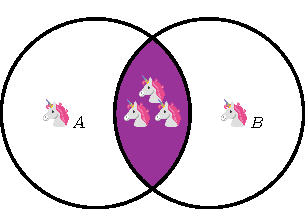
\includegraphics{images/horse_venn.pdf}
    \caption{Horses $A$ and $B$, with all the rest of the horses lying in the violet region common to both sets.}
    \label{fig:horse}
\end{figure}




\subsection*{Question 3: Insertion Sort (6+4=10 points)}

Recall the {\sc Insertion-Sort} algorithm discussed in the lecture:
\begin{code}
	{\sc Insertion-Sort}$(A,n)$\\
	1. \> \For $j=2$ \To $n$\\
	2. \> \> $key=A[j]$\\
	3. \> \> $i=j-1$\\
	4. \> \> \While $i>0$ and $A[i]>key$\\
	5. \> \> \> $A[i+1]=A[i]$\\
	6. \> \> \> $i=i-1$\\
	7. \> \> $A[i+1]=key$
\end{code}

\noindent
In the lecture, you have seen a correctness proof of the algorithm based on the following loop invariant for the (outer) for loop:
\begin{itemize}
	\item Let $A_j[1,\ldots,n]$ denote the array at the beginning of iteration $j$ (end of iteration $j-1$). We have that $A_j[1,\ldots,j-1]$ stores the same values as $A[1,\ldots,j-1]$ but in sorted order, while $A_j[\ell] = A[\ell]$ for $j \leq \ell \leq n$. 
\end{itemize}
In this problem, you will fill in a bit more detail in the proof, by also introducing a loop invariant for the (inner) while loop. You will use the following loop invariant:
\begin{itemize}
	\item Let $A_{j,i}[1,\ldots,n]$ denote the array at the beginning of iteration $i$ of the inner loop (for $0 \leq i \leq j-1$). 
    Then:
    \begin{itemize}
        \item If the loop executes with value $i+ 1$, then 
        \begin{enumerate}[nosep]
		\item $A_{j,i}[1,\ldots,i] = A_j[1,\ldots,i]$, and
		\item If $i+2 \leq j$, then $A_{j,i}[i+2,\ldots,j] = A_j[i+1,\ldots,j-1]$ and $A_j[j] < A_{j,i}[i+2]$.
	\end{enumerate}
 \item Otherwise (if the while loop terminates before reaching value $i + 1$), then $A_{j,i} = A_{j,i+1}$.
    \end{itemize}

\end{itemize}

Solve the following tasks:
\begin{enumerate}
	\item Prove the while loop invariant above using induction over $i$. Start your base case at $i=j-1$ and use backwards induction to show that the claim holds for all smaller $i$. (Prove this for an arbitrary value of $j$,
 where $1 \leq j \leq n$.)
	
\begin{solution}   INSERT YOUR SOLUTION HERE   \end{solution}
	
	\item Use the inner loop invariant to show the induction step of the outer loop invariant.
	
\begin{solution}   INSERT YOUR SOLUTION HERE   \end{solution}
	
\end{enumerate}

